% mnras_template.tex
%
% LaTeX template for creating an MNRAS paper
%
% v3.0 released 14 May 2015
% (version numbers match those of mnras.cls)
%
% Copyright (C) Royal Astronomical Society 2015
% Authors:
% Keith T. Smith (Royal Astronomical Society)

% Change log
%
% v3.0 May 2015
%    Renamed to match the new package name
%    Version number matches mnras.cls
%    A few minor tweaks to wording
% v1.0 September 2013
%    Beta testing only - never publicly released
%    First version: a simple (ish) template for creating an MNRAS paper

%%%%%%%%%%%%%%%%%%%%%%%%%%%%%%%%%%%%%%%%%%%%%%%%%%
% Basic setup. Most papers should leave these options alone.
\documentclass[a4paper,fleqn,usenatbib]{mnras}

% MNRAS is set in Times font. If you don't have this installed (most LaTeX
% installations will be fine) or prefer the old Computer Modern fonts, comment
% out the following line
\usepackage{newtxtext,newtxmath}
% Depending on your LaTeX fonts installation, you might get better results with one of these:
%\usepackage{mathptmx}
%\usepackage{txfonts}

% Use vector fonts, so it zooms properly in on-screen viewing software
% Don't change these lines unless you know what you are doing
\usepackage[T1]{fontenc}
\usepackage{ae,aecompl}

%%%%% AUTHORS - PLACE YOUR OWN PACKAGES HERE %%%%%

% Only include extra packages if you really need them. Common packages are:
\usepackage{graphicx}	% Including figure files
\usepackage{amsmath}	% Advanced maths commands
\usepackage{amssymb}	% Extra maths symbols
\usepackage[xindy]{glossaries}
\glsdisablehyper

%%%%%%%%%%%%%%%%%%%%%%%%%%%%%%%%%%%%%%%%%%%%%%%%%%

%%%%% AUTHORS - PLACE YOUR OWN COMMANDS HERE %%%%%

% Please keep new commands to a minimum, and use \newcommand not \def to avoid
% overwriting existing commands. Example:
%\newcommand{\pcm}{\,cm$^{-2}$}	% per cm-squared

\newcommand{\GSF}[1]{\noindent\textcolor{blue}{GSF:#1}}

\makeglossaries

%glossary
\newacronym{alfa}{ALFA}{Arecibo L-Band Feed Array}
\newacronym{dm}{DM}{Dispersion Measure}
\newacronym{frb}{FRB}{Fast Radio Burst}
\newacronym{fwhm}{FWHM}{Full-Width at Half-Maximum}
\newacronym{gbt}{GBT}{Greenbank Telescope}
\newacronym{igm}{IGM}{Intergalactic Medium}
\newacronym{ism}{ISM}{Interstellar Medium}
\newacronym{nip}{NIP}{Non-image Processing}
\newacronym{paf}{PAF}{Phased-Array Feeds}
\newacronym{rfi}{RFI}{Radio-frequency Interference}
\newacronym{ska}{SKA}{Square Kilometre Array}
\newacronym{sefd}{SEFD}{System Equivalent Flux Density}
\newacronym{snr}{SNR}{Signal-to-Noise Ratio}
\newacronym{sps}{SPS}{Single Pulse Search}
\newacronym{vlbi}{VLBI}{Very Long Baseline Interferometry}

%%%%%%%%%%%%%%%%%%%%%%%%%%%%%%%%%%%%%%%%%%%%%%%%%%

\title[ALFABURST Initial]{ALFABURST Initial}

\author[ALFABURST Team]{
ALFABURST Team
}

% These dates will be filled out by the publisher
\date{Accepted XXX. Received YYY; in original form ZZZ}

% Enter the current year, for the copyright statements etc.
\pubyear{2017}

% Don't change these lines
\begin{document}
\label{firstpage}
\pagerange{\pageref{firstpage}--\pageref{lastpage}}
\maketitle

% Abstract of the paper
\begin{abstract}
% What is the point of the paper?
% What is the context of the study? What background information is necessary to understand the study?
% How was the study done?
% What is the main take away message?
% What can be said about these results, and how does this affect future work?
The ALFABURST fast radio burst (FRB) survey has been observing commensally with
other projects using the ALFA receiver since July 2015. We report on the
non-detection of any FRBs from that time until June 2017. With current FRB rate
models we expected to see multiple FRBs based on the total observing time,
telescope sensitivity and beam size. We discuss the implications for this
non-detection FRBs in the context of recent detections with other telescopes.
\end{abstract}

% Select between one and six entries from the list of approved keywords.
% Don't make up new ones.
\begin{keywords}
radio continuum: transients -- methods: observational
\end{keywords}

%%%%%%%%%%%%%%%%%%%%%%%%%%%%%%%%%%%%%%%%%%%%%%%%%%

\section{Introduction}
\label{sec:intro}

As of August 2017, 23 \glspl{frb} have been reported
\citep{2016PASA...33...45P}. The majority of which have been detected with the
Parkes Radio Telescope at L-Band frequencies. FRB121102 was detected in the
PALFA survey using Arecibo Observatory, showing \glspl{frb} are not a phenomenon
local to the Parkes Telescope \citep{2014ApJ...790..101S}. This \gls{frb} is the
only known \gls{frb} to repeat \citep{2016ApJ...833..177S}.  FRB110523 was
detected with the Green Bank Radio Telescope at UHF frequencies, confirming
\glspl{frb} occur at other radio frequencies \citep{2015Natur.528..523M}.
Recently, a number of very bright \glspl{frb} have been detected with UTMOST
\citep{2017MNRAS.468.3746C} and ASKAP \citep{2017ApJ...841L..12B}.

The population of \glspl{frb} varies significantly across the parameter space.
The measured \glspl{dm} varies from 278 (FRB160410) to 1629 (FRB121002), with
pulse widths ranging from sub-millisecond unresolved to 10's of milliseconds,
and apparent flux densities covering 4 orders of magnitude. The sky distribution
of these sources is preferentially at high galactic latitudes
\citep{2015MNRAS.451.3278M}.

So far, \glspl{frb} have been poorly localized as most have been detected with
single dish telescopes. The unknown detection position in the beam, and one-off
nature of \glspl{frb} does not allow determination of the absolute flux or
spectral index. Only the repeater FRB121102 has been localized using \gls{vlbi}
\citep{2017ApJ...834L...8M, 2017ApJ...834L...7T}. Localization is a key
observable which needs to be improved in order to identify the source
environment. Which requires use of interferometric arrays for arc-minute
localization. Arrays such as CHIME, MeerKAT and ASKAP will provide such
localization.

Other than localization, more of the frequency space is being searched. Low
frequency searches with LOFAR \citep{2015MNRAS.452.1254K}, MWA
\citep{2015AJ....150..199T}, and the GBT \citep{2017arXiv170107457C} have
reported non-detections.  No large surveys for \glspl{frb} have been done above
L-band frequencies. This is, in part, due to the narrowing of beam size which
limits sky coverage.  \cite{2017arXiv170507553L} ran a coordinated-in-time,
multi-telescope campaign of the repeater \gls{frb}.  They report non-detection
of pulses at VHF, C-band, Ku-band during periods of detected bursts in L-band
and S-band.

For single dish telescopes there is a trade-off of sensitivity to sky coverage.
Small beams, while providing a large sky coverage, have been unsuccessful at
detecting \glspl{frb}. Conversely, Arecibo provides the highest sensitivity, but
with a very narrow beam. Parkes appears to be near the optimal trade-off point
between sensitivity and beam size.  ASKAP dishes with \glspl{paf} provides a
large sky coverage with a significant enough sensitivity to detect bright
\glspl{frb}. Interferometric arrays such as CHIME and MeerKAT while provide both
sensitivity and sky coverage.

%(needs more additions)
%
%The first FRB~\citep{2007Sci...318..777L} was detected in a reprocessing of
%data from a survey of the Magellanic Clouds~\citep{2006ApJ...649..235M}, with
%an estimated flux density of $30\pm10$~Jy. The detection of this event led to a
%spurt in single pulse searches, conducted on both archival data
%(burke-spolaor?) as well as data from surveys specially designed to look for
%such events. \citet{2012ApJ...744..109S} conducted a wide-field survey using
%the Allen Telescope Array, in which each of the forty two antennas of the array
%was pointed in a different direction. Although this configuration rendered the
%limiting fluence high ($\sim$111~kJy~$\mu$s), it allowed a large field of view
%($\sim$147~deg$^2$). The survey resulted in no detection, and yielded an event
%rate of 2~sky$^{-1}$~hr$^{-1}$ for 10~ms-wide pulses with flux density greater
%than 44~Jy.
%
%
%\subsection{Repeater (needs editing)}
%FRB121102 was discovered in the Pulsar- ALFA (PALFA) survey as a highly
%disperesed bright single radio pulse in beam 4 with a dispersion measure (DM)
%of ~559 $\rm cm^{-3}~pc$. The results of the single pulse detection were
%published in~\cite{2014ApJ...790..101S}. The authors also compute a FRB rate
%based on the single detection. Based on the numerical model of the ALFA beams,
%they obtained a Field of View (FoV) weighted gain of the system and the
%instantaneous FoV. The total time on sky was computed as the difference of
%total observation time and total data masked due to Radio Frequency
%Interference (RFI). Thus, assuming Poisonnian statistics for the FRB rate, they
%compute the best FRB rate for the computed flux sensitivity of PALFA. They also
%report FRB rate for flux sensitivity corresponding to a gain  greater than 0.4
%K~$\rm Jy^-1$ which corresponds to the average gain of the Parkes multi-beam
%receiver. After the initial discovery, more radio follow-up was carried out
%with no detections at any of the epochs. The follow-up continued into the next
%year when~\cite{2016Natur.531..202S} reported the discovery of 10 new bursts in
%2015. The bursts had the same DM as the discovery burst and the detections were
%within a few arc seconds from the initial detection suggesting that the later
%pulses came from the same source. The authors were unable to find a period for
%the bursts and also discuss the possiblity that these could be RFI though all
%the observational evidence suggests that the source is astrophysical.
%
% This discovery generated a lot of interst in multi-wavelength
%follow-up efforts.~\cite{2016ApJ...833..177S} report the first multi-wavelength
%follow-up results where seven more bursts were detected, all in radio and two
%from the Green Bank Telescope taking the total to 17 pulses. They reported an
%interesting frequency structure the pulses have which varies on a pulse to
%pulse basis.~\cite{2016Natur.531..202S} had already showed that the pulses had
%peculiar frequency behaviour which cannot be explained by scintillation effects
%in the ISM and the IGM. This alongwith the large range of spectral indices
%($-$13 -- 5) observed in the bursts led the authors to believe that the
%emission variability is intrinsic to the source. The discovery of repeating
%bursts led to a massive campaign using the Very Large Array (VLA) in order to
%detect and localize the FRB to arcsecond precision.~\cite{2017Natur.541...58C}
%reported a successful localization of FRB 121102 with the final position of the
%burst with an error of 100~mas. Such precise localization made discovery of a
%counterpart plausible. The paper also reports a discovery of a persistent radio
%source which is offset by $\sim$12~mas from the point
%source.~\cite{2017ApJ...834L...8M} make a strong argument for the association
%for the persistent radio source and the FRB based on high resolution European
%VLBI Network (EVN) observations and also report that the flux variation of the
%radio source are unlike what would be expected from an Active Galactic
%Nuclei.~\cite{2017ApJ...834L...7T} presented the results of the detection of an
%optical counterpart associated with the radio source and thus with the FRB.
%Based on the spectrum of the optical source, tehy conclude that it is a mag
%25.5AB starforming dwarf galaxy with a total mass of $7 \times$10$^{7}~\rm
%M_{\odot}$. They also argue that though the optical signatures are unlike any
%seen from an AGN with optical counterparts, a lot of AGNs are discovered where
%the optical counterpart is absent and hence no claims on the radio source can
%be made. They also suggest that localizing such repeater source would be easier
%if the field was searched for optical spectra similar to the one shown by this
%source. The big assumption here is that there is a strong relationship between
%the FRB and the type of hosts where they are found.

\section{ALFABURST Overview}
\label{sec:overview}

ALFABURST is an \gls{frb} search instrument which has been used to commensally
observe since July 2015 with other \gls{alfa} observations at Arecibo
Observatory. This system is a component of the SETIBURST back-end
\citep{2017ApJS..228...21C} and uses ARTEMIS \citep{2015MNRAS.452.1254K} for
automated, real-time detection. During this time period an \gls{sps} was
performed from \gls{dm} 0 to 10000, pulse width from $256 \mu s$ to $16$ ms,
across a 56 MHz bandwidth for all 7 beams. We choose this \gls{dm} limit as it
can be approximately associated with a redshift that is far beyond our
sensitivity limits as discussed in Section \ref{sec:event_rates}. The gain of
Arecibo allows for the most sensitive \gls{frb} search to date.

Detections above an \gls{snr} of 10 were recorded along with an $8.4$ second
dynamic spectrum window around the event. If multiple events were detected in
the same time window, these events were pooled together.  Approximately 150k
windows were recorded between July 2015 and June 2017, the vast majority of
which are false detections due to \gls{rfi} signals passing through the
real-time \gls{rfi} exciser. We detect no \glspl{frb} in our commensal survey.

A wide-feature, learned model was used to classify the event windows in order to
filter out \gls{rfi} and create a priority queue for visual examination. This
model and the post-processing procedures are discussed in Section
\ref{sec:event_classify}. We discuss the expected event rates in Section
\ref{sec:event_rates} and consider possible explanations for our non-detection
result in Section \ref{sec:discuss}.

%%% SYSTEM VERIFICATION BEGINS %%%

\subsection{System Verification}
\label{sec:system_verify}

PALFA survey scheduling includes regularly observing known pulsars to verify
timing analysis, this provides a consistent verification of our \gls*{sps} to
detect pulses. As the PALFA survey is performed in the galactic plane a number
of high \gls*{dm} pulsars were observed, single pulses from B1859+03 (\gls*{dm}:
402), B1900+01 (\gls*{dm}: 245) (Figure \ref{fig:B1900}), B2002+32 (\gls*{dm}:
234), B1933+16 (\gls*{dm}: 158), among others were detected.

% alfaburst-initial-survey/notebooks/B1900_01.ipynb
\begin{figure}
    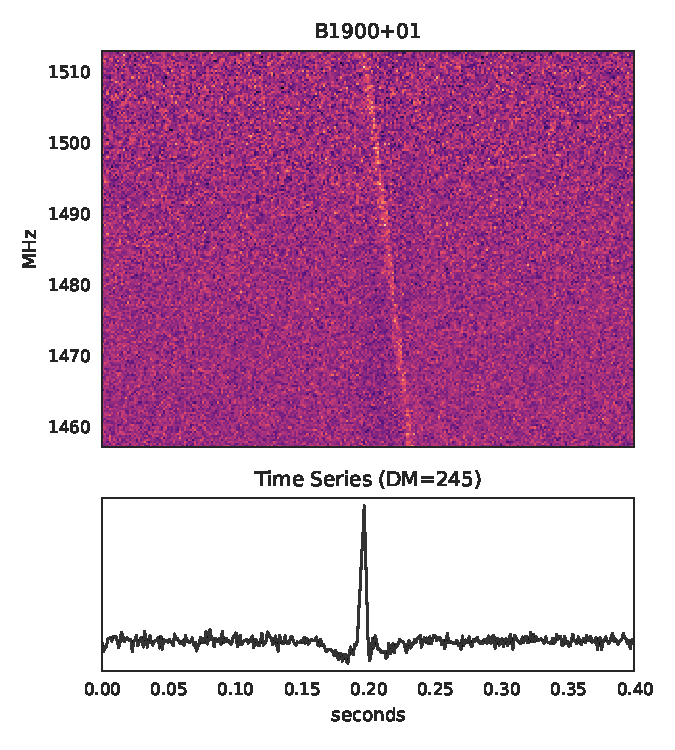
\includegraphics[width=1.0\linewidth]{figures/B1900_01.pdf}
    \caption{Detection of a single pulse from Pulsar B1900+01 (DM 245). The
    baseline dip before and after the pulse is due to zero-DM removal.
    }
    \label{fig:B1900}
\end{figure}

%%% SYSTEM VERIFICATION ENDS   %%%

%%% OBSERVATION TIME BEGINS %%%

\subsection{Observing Time}
\label{sec:obs_time}

From the beginning of July 2015 to the end of June 2017 \gls*{alfa} has been
used for approximately 1400 hours of observing, with all seven beams functional.
Due to pipeline development and hardware reliability ALFABURST was active and
functional for, on average, 322 hours per beam.  The current system is setup to
be reliably in use for all beams any time \gls*{alfa} is active and in the
correct receiver turret position. Of the survey coverage, approximately 65\% of
the time has been in pointings out of the galactic plane ($|b| > 5^{\circ}$).
These pointings are primarily from to the ongoing AGES survey.  Pointings in the
plane are primarily from the PALFA survey. The PALFA continues to do a \gls{sps}
for \glspl{frb} across the full band. This provides an independent search
pipeline to ALFABURST for these observations. Since the beginning of ALFABURST
observations no \glspl{frb} have been reported by PALFA.  Since we are searching
up to a \gls{dm} of 10000 the survey is still sensitive to \glspl{frb} at
cosmological distances when observing in the galactic plane. But, scintillation
effects can reduce the overall \gls{frb} event rates
\citep{2015MNRAS.451.3278M}.

%%% OBSERVATION TIME ENDS   %%%

%%% SKY COVERAGE BEGINS %%%

\subsection{Survey Coverage}
\label{sec:survey_coverage}

Since ALFABURST was installed, the majority of ALFA observation time is
allocated for the AGES \citep{2006MNRAS.371.1617A} and PALFA
\citep{2006ApJ...637..446C} surveys (Figure \ref{fig:sky_coverage}).  The AGES
survey pointing is off the galactic plane, thus there is little dispersion and
scattering due to the galactic \gls*{ism}. PALFA is a pulsar search survey with
pointings near the galactic plane. These lines of sight can introduce
significant dispersion due to the \gls*{ism}. We search out to a DM of 10000
which is well beyond the maximum galactic dispersion, even when \gls*{igm}
dispersion is accounted for from sources of cosmological distances. The PALFA
survey detected the repeating \gls{frb} FRB121102 \citep{2014ApJ...790..101S},
the only \gls{frb} detected with Arecibo thus far. As ALFABURST has been running
commensally with the PALFA survey since 2015 these two backends act as
independent \gls{sps} pipelines, useful for detection verification.

% alfaburst-initial-survey/notebooks/Sky_Coverage.ipynb
\begin{figure*}
    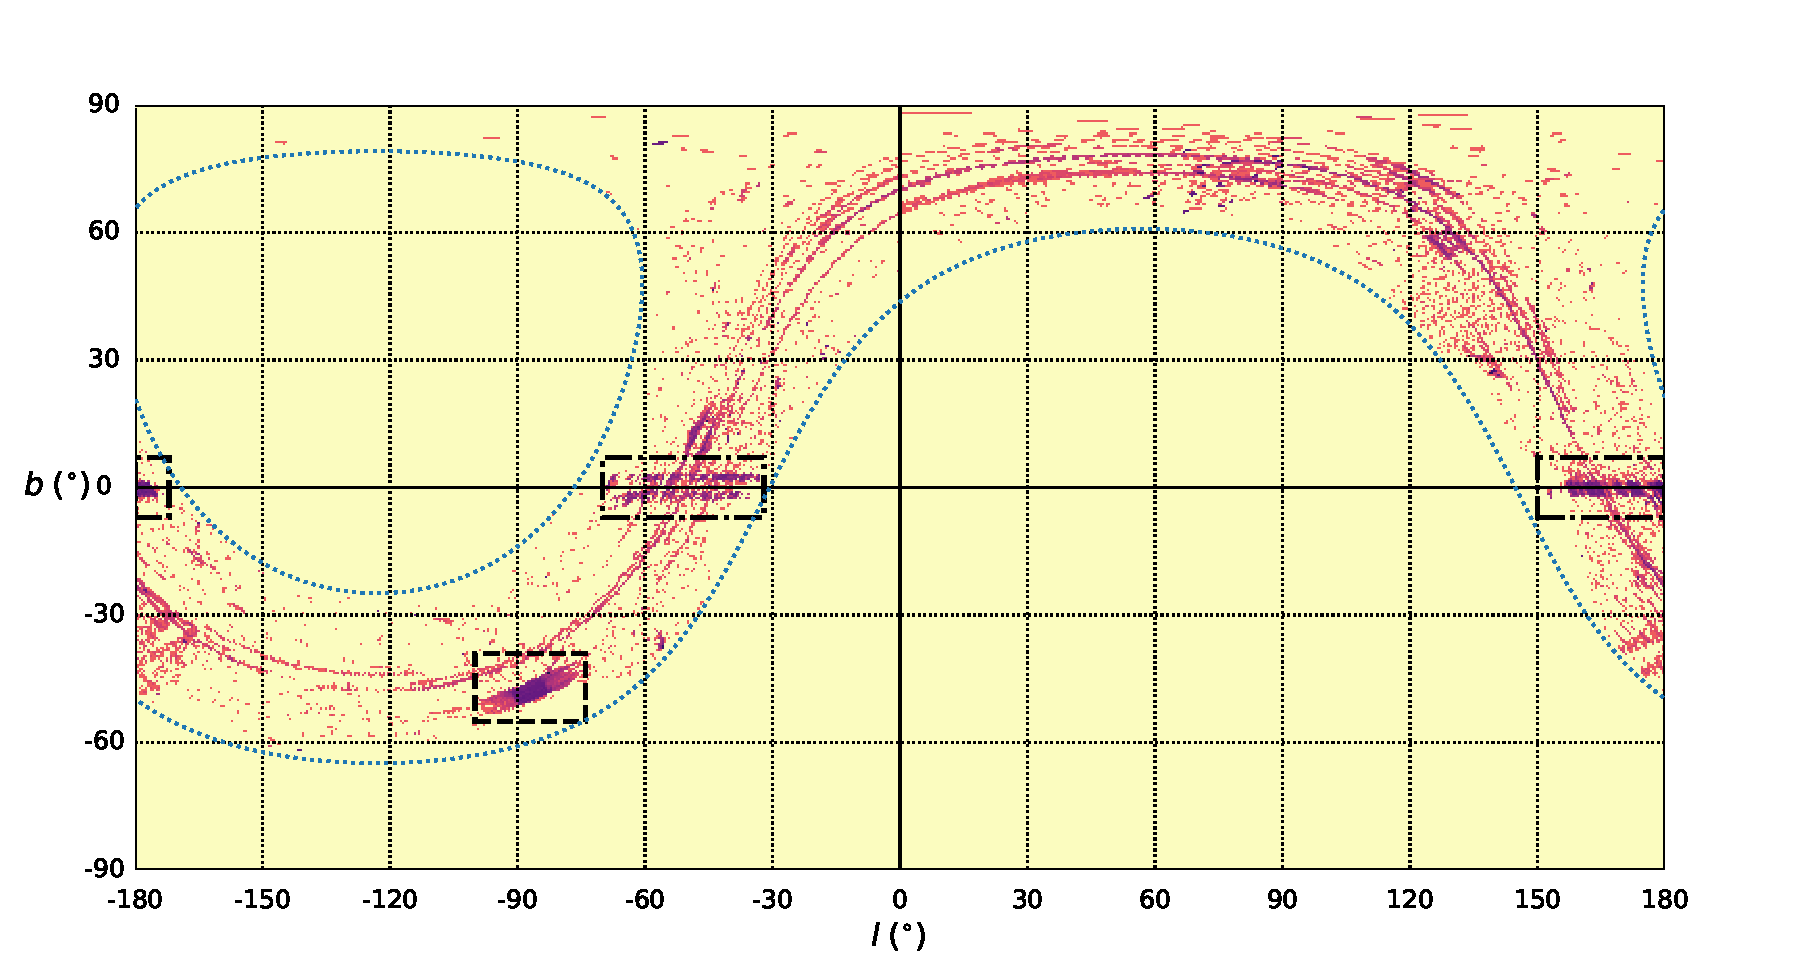
\includegraphics[width=1.0\linewidth]{figures/cartview_sky_coverage.pdf}
    \caption{Sky coverage during ALFA usage between July 2015 and June 2017,
    shown in a Cartesian projection in galactic coordinates. Color represents
    total time pointing in a log scale. The majority of ALFA usage during this
    time was for the PALFA survey along the galactic plane (dot-dashed boxes)
    and the AGES survey (dashed box).  The S-shaped arcs across the plot are due
    to fixed pointings in local azimuth and altitude.
    }
    \label{fig:sky_coverage}
\end{figure*}

%%% SKY COVERAGE ENDS   %%%

%%% PRIORITIZER BEGINS %%%

\section{Event Prioritization and Classification}
\label{sec:event_classify}

% TODO
% Event Classification and Prioritization
%   * priority classifier model
%       * labelled data
%       * wide feature selection + classifier
%       * deep feature selection + classifier
%   * event statistics

%%% PRIORITIZER ENDS   %%%

%%% EVENT RATES BEGINS %%%

\section{Expected FRB Event Rates}
\label{sec:event_rates}

As of this writing, only 23 \glspl{frb} have been reported. As these events vary
significantly in \gls{dm}, pulse width, and flux density we assume a simple
model to derive an expected event rate with our survey.  We use a model
\citep{2013MNRAS.436L...5L} which assumes \gls{frb} sources are standard candles
with a fixed spectral index, uniformly distributed in comoving volume. The
events rates in this model are scaled to the event rates reported in
\cite{2013Sci...341...53T}.

We use two beam models to derive our expected rates. The first is a simple
\gls{fwhm} beam size with a fixed sensitivity limit that allows us to sample a
constant co-moving volume. We also use a model which accounts for the \gls{alfa}
first side lobes. This results in a sky coverage and sensitivity which varies as
a function of beam gain. This model results in a higher expected event rate than
the simple \gls{fwhm} model. We use this full beam model as the Arecibo dish
provides high sensitivity at the cost of a smaller beam size. The side lobes of
the \gls{alfa} feed would be sensitive to many of the previously detected
\glspl{frb}. By including the full beam we improve our survey coverage while
still being sensitive to these brighter \glspl{frb}.

\subsection{FWHM Beam}
\label{sec:fwhm_beam_rates}

An \gls*{alfa} beam is approximately 3.8' x 3.3' at \gls*{fwhm} across the band.
Given the average observing time per beam of 322 hours this results in a survey
coverage of $6.2 \; \textrm{deg}^2 \; \textrm{hours}$ when accounting for all 7
beams. This is a small survey coverage compared to most other \gls{frb} surveys,
primarily due to the narrow beam size of Arecibo. ALFABURST does not compete
with other surveys on sky coverage, rather it is the highest sensitivity
\gls{frb} survey to date.  Using Equation 6 of \cite{2015MNRAS.452.1254K}, an
\gls*{sps} pipeline is sensitive to pulses with a minimum flux density (in Jy)
of
%
\begin{equation}
S_{min} = \textrm{SEFD} \frac{\textrm{SNR}_{min}}{\sqrt{D \; \Delta \tau \;
\Delta \nu}}
\end{equation}
%
which is a function of the telescope \gls*{sefd}, the minimum \gls*{snr}
detection level $\textrm{SNR}_{min}$ and the decimation rate $D$ compared to the
native instrumental time resolution $\tau$, this comes from the search pipeline
which averages together spectra to search for scattered pulses. ALFABURST has a
native resolution of $\Delta \tau = 256 \; \mu s$, effective bandwidth $\Delta
\nu = 56 \textrm{MHz}$, and $\textrm{SNR}_{min} = 10$. The \gls*{sefd} of the
\gls*{alfa} receiver is approximately 3 Jy across the band for all beams.

The \gls{sps} pipeline is configured to search for pulses from 256 $\mu$s to 16
ms. Assuming a matched filter this results in a sensitivity to pulses with a
minimum flux of $S_{256 \mu\textrm{s}} = 250$ mJy to $S_{16 \; \textrm{ms}} =
31$ mJy. Figure \ref{fig:fwhm_sefd_z} shows the peak flux density of using the
standard candle \gls{frb} model as a function of source redshift for different
model spectral indices. The dashed lines of constant flux is the sensitivity of
the ALFABURST search pipeline to pulses of different widths. Assuming a positive
spectral index model ($\alpha=1.4$) results in a sensitivity out to the maximum
redshift /\gls{dm} for pulses with widths of at least 1 ms. A flat spectral
index model results in sensitivity from $z \sim 1.5$ out to $z \sim 5$ depending
of pulse width. A negative spectral index model ($\alpha \sim -1.4$) limits the
survey to $z < 3$.

% alfaburst-initial-survey/notebooks/ALFABURST_Derived_FRB_Rates.ipynb
\begin{figure}
    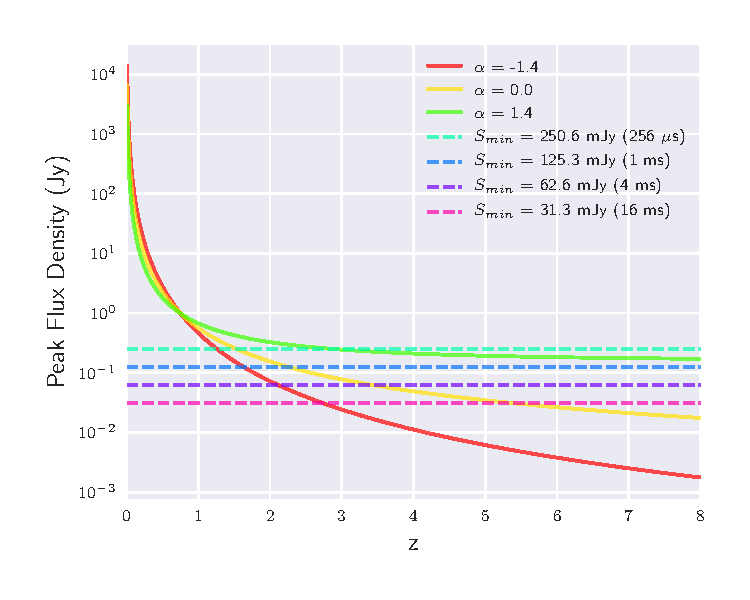
\includegraphics[width=1.0\linewidth]{figures/fwhm_sefd_z_relation.pdf}
    \caption{Sensitivity of the ALFABURST search pipeline (dashed) to FRB pulses
    assuming a standard candle model using different spectral index models
    (solid).
    }
    \label{fig:fwhm_sefd_z}
\end{figure}

We will assume a simple model of $\alpha=0$ as we have limited information about
the source spectral index. And, we will use a pulse width of 4 ms as that is an
approximate median pulse width of reported \glspl{frb}. This results in a
maximum redshift of $z=3.4$ (a co-moving distance of 6.8 Gpc) and a survey volume
of $4.2 \times 10^6$ Mpc$^3$ when using all 7 \gls{alfa} beams. The number of
galaxies sampled in this volume is $4 \times 10^5$ assuming a constant galaxy
number density of $10^{-2}$ per Mpc$^3$.  The volumetric event rate from
\cite{2013Sci...341...53T} is stated to be $R_{\textrm{FRB}} = 10^{-3}$
\glspl{frb} per galaxy per year. We should expect to detect $\sim 1.5$
\glspl{frb} based on the current observation time.

\subsection{Primary Beam and First Side Lobes}
\label{sec:full_beam_rates}

In Section \ref{sec:fwhm_beam_rates} we are only take into account the beam
size out to the \gls{fwhm}. We can take into account the entire first side lobes
of the beams as Arecibo would be sensitive to detect most previous
\glspl{frb} in the first side lobes. Using the parameterized \gls{alfa} beam
model (Figure \ref{fig:alfa_beam}) \citep{GALFAbeam} we can compute the
\gls{frb} survey metric and expected rates as a function of beam sensitivity.
The first side lobes peak at around $-10$ dB and provide a significant increase
in sky coverage compared to just the primary lobes.

% alfaburst-initial-survey/notebooks/ALFABURST_Derived_FRB_Rates.ipynb
\begin{figure}
    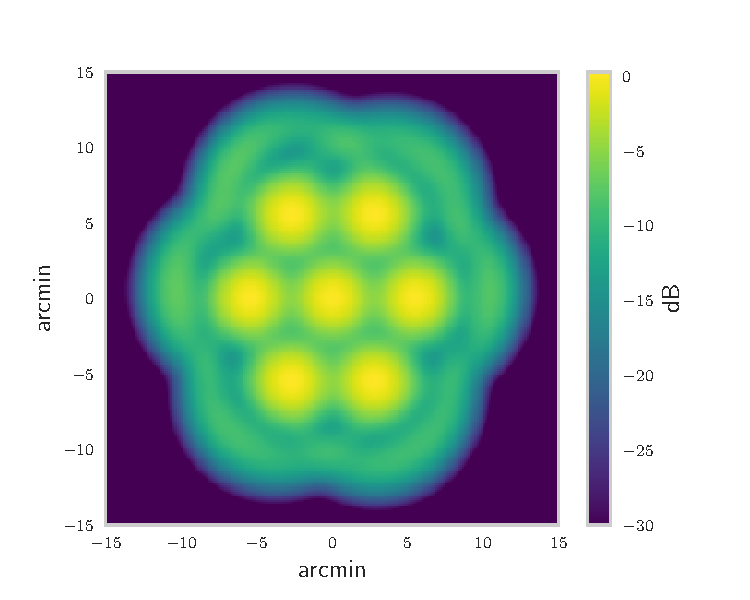
\includegraphics[width=1.0\linewidth]{figures/ALFA_beam_1425MHz_dB.pdf}
    \caption{Primary and first side lobe model of the AFLA receiver in
    decibels, cut-off at $-30$ dB.The first side lobe peak at around $-9$ dB.
    }
    \label{fig:alfa_beam}
\end{figure}

The total survey metric can be computed as a function of the beam sensitivity by
integrating over the beam (Figure \ref{fig:survey_metric_sense}). The flux
threshold has been set by assigning the $-3$ dB the same sensitivity as the
\gls{fwhm} sensitivity. The segment which increased the survey metric to
approximately $20 \; \textrm{deg}^2$ hours is due to including more of the
primary beam beyond the \gls{fwhm} point. The steep increase in the survey
metric is from including the first side lobes. The long tail is from the residual
sensitivity by integrating over the remaining beam.

% alfaburst-initial-survey/notebooks/ALFABURST_Derived_FRB_Rates.ipynb
\begin{figure}
    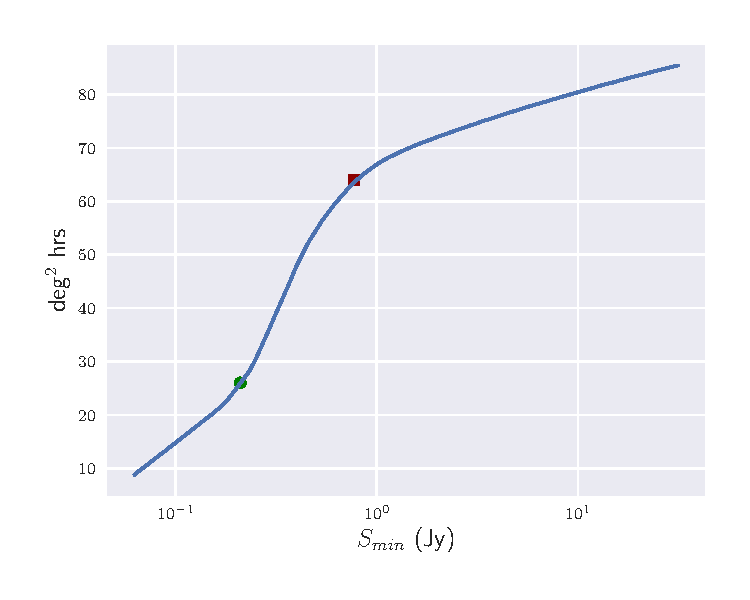
\includegraphics[width=1.0\linewidth]{figures/full_survey_metric_sense.pdf}
    \caption{Survey metric as a function of the ALFA receiver minimum
    sensitivity using the ALFA primary and first side lobes.
    }
    \label{fig:survey_metric_sense}
\end{figure}

The significant increase in the survey metric only modestly improves our survey
volume. Plotting the survey metric as a function of maximum redshift (Figure
\ref{fig:full_sefd_z}) shows that the full beam model increases the survey
volume out to $z<1.5$. Including additional ALFA side lobes would have minimal
increase in the survey volume.

% alfaburst-initial-survey/notebooks/ALFABURST_Derived_FRB_Rates.ipynb
\begin{figure}
    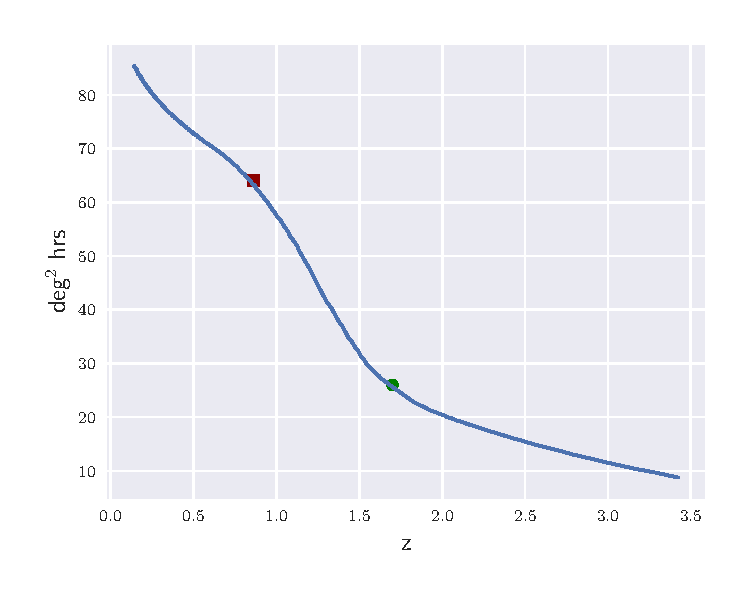
\includegraphics[width=1.0\linewidth]{figures/full_sefd_z_relation.pdf}
    \caption{Survey metric as a function of redshift using the standard candle
    model with a flat spectral index ($\alpha=0$) and pulse width of 4 ms. The
    bump out to $z=1.5$ is due to the including the ALFA first side lobes.
    }
    \label{fig:full_sefd_z}
\end{figure}

Accounting for this extra survey coverage results in an integrated survey volume
of $5.8 \times 10^6$ Mpc$^3$. The expected number of \glspl{frb} in the survey is
$\sim 2$ when using the same galaxy number density and $R_{\textrm{FRB}}$ as
Section \ref{sec:fwhm_beam_rates}.

\subsection{Sensitivity Upper Limit}
\label{sec:upper_limit}

Part of the \gls{sps} pipeline is a parameterized \gls{rfi} exciser. The choice
of these parameters sets an upper limit on the flux of a pulse before it a
portion of the flux is clipped and replaced. Individual frequency channels in a
spectra are replaced when they exceed a threshold $T_{\textrm{chan}}$ after the
spectra is normalized ($\mu=0$, $\sigma=1$). And, entire spectra are clipped
when the summed spectra exceeds a threshold $T_{\textrm{spectra}}$. For standard
ALFABURST operation $T_{\textrm{chan}} = 5$ and $T_{\textrm{spectra}} = 10$.

For very bright, small \gls{dm} pulses the \gls{rfi} exciser will replace
channels or spectra, reducing the overall flux or potentially removing the
entire pulse.  For bright, high \gls{dm} pulses the spectra will likely not be
replaced, but individual channels may be, resulting in a lower detected flux.
The \gls{rfi} exciser only works in the undecimated-in-time case ($D=1$), that
is the sensitivity that we are most concerned about when setting the \gls{rfi}
exciser thresholds.

\glspl{frb} detected at L-Band range between 200 mJy to a few Jy in flux
density, typically on the order of 5-10 milliseconds. For the sensitivity of the
\gls{alfa} receiver, individual channels of flux greater than 2.8 Jy will be
flagged, this will not have an effect on our ability to detect even the
brightest \glspl{frb}.  The maximum integrated pulse flux ($256 \mu$s width,
\gls{dm}$=0$) is $\sim250$ mJy before the pulse is clipped. The maximum
detectable flux increases as the square-root of the pulse width.  We see in
verification observations of bright, low \gls{dm} pulsars that individual
pulses are often excised. But, as we are interested in detecting high \gls{dm}
\glspl{frb} we have a higher upper limit as the flux is spread over multiple
spectra.

For reference the minimum \gls{dm} of a pulse before the at least one channel is
shifted to the next spectra in time is \gls{dm}$=1.8$ for the typical ALFABURST
observing band (using Eq. 5.1 of \cite{2004hpa..book.....L}). And, the minimum
\gls{dm} before each frequency channel is in a separate spectra is
\gls{dm}$=976$. Most reported \glspl{frb} fall with in this \gls{dm} range, so
we consider a test \gls{frb} with a dispersion measure of 250 and narrow
pulse width of $256 \mu$s to report our survey upper-limit sensitivity. A
\gls{dm} of 250 results in approximately $1/128$ of the pulse per spectra. A
bright pulse ($>32$ Jy) would be excised as \gls{rfi} in this test case. This an
extreme case, as most \glspl{frb} are wider in width and at higher \glspl{dm}.
Our pipeline would not excise all detected \glspl{frb} except the extreme
FRB150807.  This also assumes the \gls{frb} is detected at boresight, we would
still be sensitive to such bright pulses in the side lobes. Figure
\ref{fig:fluence_rate} shows that ALFABURST sensitivity region based on pulse
width and peak flux, assuming detection at boresight.

% alfaburst-initial-survey/notebooks/Fluence_Rate.ipynb
\begin{figure}
    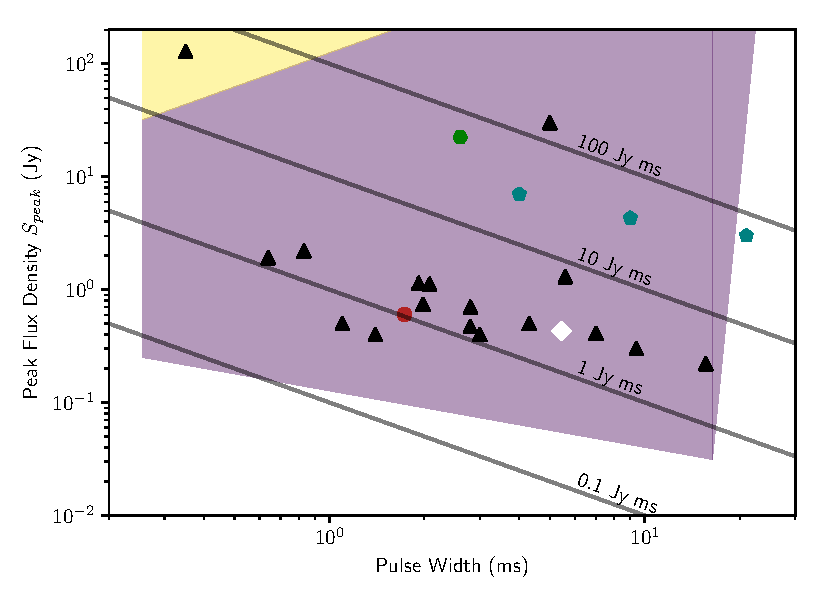
\includegraphics[width=1.0\linewidth]{figures/fluence_rate.pdf}
    \caption{ALFABURST single pulse sensitivity (purple region) improves upon
    the sensitivity of all past FRB surveys. Automated RFI excision excludes
    narrow in width, low DM, bright FRBs such as FRB150807 (yellow region).
    Previously detected FRBs from Parkes (black triangle), GBT (red circle),
    Arecibo (white diamond), UTMOST (cyan pentagon), and ASKAP (green hexagon)
    are plotted for reference.
    }
    \label{fig:fluence_rate}
\end{figure}

%%% EVENT RATES ENDS   %%%

%%% FLUENCE RATE BEGINS %%%

\subsection{Fluence Rate}
\label{sec:fluence}

% TODO: Keane and Petroff fluence rate, plot
% Keane & Petroff 2014 - fluence completeness
% compare to fluence rate to previous surveys

%%% FLUENCE RATE ENDS   %%%

\section{Discussion}
\label{sec:discuss}

% TODO
% discount scintillation effects (Macquart and Johnston)
% Spectral Index constraints
% Possible reasons: star formation rate, scintillation, steep spectrum
%   * Star formation rate:
%       * implied FRB Luminosity function: cosmological star formation rate, peaks
%       around z=2? write notebook to produce rates, Madau & Dickinson 2014
%   * scintillation:
%       * limited bandwidth, repeater band varies
%       * relation to Macquart and Johnston paper: rate off/on the plane is
%       different due to scintillation regimes
%       * repeater and low freq frb searches: spectra are not pulsar like. may be
%       due to strong scintillation
%   * steep spectrum/band limited:
%       * relation to ASKAP detections
%       * Law et al see no detections at low and 5 GHz+ freqs -> band limited,
%       steep spectrum ; we are probing a large z, perhaps the band is shifted
%       out of L-band

The limited processing bandwidth of ALFABURST may be a cause of the survey
non-detection. Multiple detected \glspl{frb} show apparent scintillation and
step spectral indicies. It is not possible to differentiate between an
apparent spectral index induced by the beam or an absolute spectral index from
the source. If an \gls{frb} did occur in the field of view of the telescope
while ALFABURST was in operation we could have been unlucky and scintillation
caused the pulse in the band to go below the detection threshold. An increase to
the full \gls{alfa} band would result in a $\sqrt{6}$ increase in sensitivity,
assuming no scintillation. This would increase our event rates to $\sim 5$
\glspl{frb} for the current amount of observation time.

\section{Future Work}
\label{sec:future_work}

The current \gls*{sps} pipeline is undergoing a significant upgrade. The input
bandwidth is limited to 56 MHz of the full 336 MHz digital band due to IO
limitations. A new pipeline developed for \gls*{ska} \gls*{nip} will be used to
process the full \gls*{alfa} band. This will increase sensitivity, and improve
detection rate if \glspl*{frb} scintillate similar to FRB121102. An improved
version of the real-time \gls*{rfi} exciser is currently being developed and
will be deployed to reduce the false detection rate. The post-processing
classifier and prioritizer model is being updated to make use of an auto-encoder
to select deep features and auto-generate classes.

Over the time period ALFABURST has been active, the use of \gls*{alfa} has
decreased as the PALFA and AGES surveys end. The 327 MHz and L-band wide feeds
are commonly used. We are generalizing the \gls*{alfa} specific \gls*{sps}
pipeline to be used when these feeds are active, increasing our survey time and
sampling a larger portion of frequency space. Additionally, our search pipeline
will be duplicated for use on the \gls*{gbt} to be commensally run with L-band
observations. 

Jupyter notebooks are hosted on our public git
repository\footnote{https://github.com/griffinfoster/ab-survey-2017}.

\bibliographystyle{mnras}
\bibliography{alfaburst.bib} 

\bsp	% typesetting comment
\label{lastpage}
\end{document}

% End of mnras_template.tex
